\documentclass[10pt,a4paper]{article}

\usepackage[margin=2cm]{geometry}
\usepackage{mymath}


\pagestyle{empty}

\begin{document}

% \textbf{Title: }
% Schrödinger Bridge Problem with Dynamic of Kinetically-Interacting Particle  \\
% \textbf{Name: } Pethai N. (6680739) \\
% \textbf{Advisor: } Prof. Chatchawan P. \\


% \clearpage



% \section*{Abstract}
%     This thesis concerns an Schrödinger Bridge problem which seeks an optimal
%     redistribution of interacting Brownian particles from observed initial to 
%     terminal distributions. Specifically, the dynamic is of reflected 
%     mean-field type on punctured interior, bounded domain $\cD \subset \bR^d$. 


% \section*{Introduction}

%     From now on, the abbreviation SB will referes to dynamic type, unless state otherwise. 

%     \paragraph{Breif History of the Schrödinger Bridge Problem}



%     \paragraph{Thesis Work Summary}


% \section{Background Materials}


% \subsection{Existing results in SB} % 2 p

%     \paragraph{Entropically Regularized SB}
%     \paragraph{Structure Solution}
%     \paragraph{Sinkhorn Recursion} (IPFP)
    
% \subsection{Numerical Method for SB} % 1 p 

% \subsection{System of dynamically-Interacting Particles} % 1p


% \section{Problem Formulation}



% \section{Fixed-Point Scheme}

% In is note that the fixed-point scheme is also similar to widely adopted scheme
% in solving coupled MFG. And additionally mirror the scheme given in [] which main 
% difference being, instead of having 1-loop, they compose 3 nested structure.
%  With additional


% As noted in \cite{calzola2023_SL_hjb_reflect}, even through SL scheme is unconditionally
% stable, the inverse CFL condition is required to ensure stability of the system in the 
% presence of Neuman boundaries. The spatial interpolation error 
% $ \mathcal{O}\left( \Delta x^{2}\right)$ must be dominated by termporal 
% reflection step $ \mathcal{O}( \Delta t)$ otherwise, for too small 
% $ \Delta t$ relative to $ \Delta x^{2}$ the reflection error accumulate over time steps.
% $\Delta t^{2} /\Delta x\rightarrow 0$ as $ (\Delta x,\Delta t)\rightarrow 0$



% \section{High-Dimensional Problems}




% \paragraph{Generalizing the SOC formulation}
%     This section interprete the SOC reformulation as a special case planning-MFG system whose 
%     cost functional is restricted to quadratic kinetic. The natural extension is to consider, 
%     nonsymmetric, translation-invariant interacting kernel with additional cost term. The 
%     advantage of fixed-point algorithm is it can be directly applied with minor modification. 















\section{Numerical Experiments}

Here the experiments are conducted on 2-dimensional domain $[0,3.0]\times [0,1.2]$ punctured by 
2 circular and 3 rounded rectangular interior holes. The initial and endpoint marginals are, 
respectively, 3 mixture of Gaussian and split uniform distribution with Gaussian decay at 
boundary. The nonlocal meanfield is Guassian function 
$E(x)=\gamma _{0} \cdot \exp\left( -\| x\| ^{2} /2\sigma _{0}^{2}\right)$ where 
$\gamma _{0} =0.02$ is strenth and length scale $\sigma _{0} =0.35$. The unstructured mesh 
is generated by \textit{Gmsh} library with constrained on maximum mesh size $h_{\text{max}}$. 
Note that there is to noticeable difference between choice of structured or unstructured mesh 
in execution time or convergence in fixed-point contraction rate. See figure \ref{fig:density_particle_2d_illustrate}
along with convergence \ref{tab:fixed_point}.

\begin{figure}[htbp]
    \centering
    \begin{subfigure}[b]{0.6\textwidth}
        \centering
        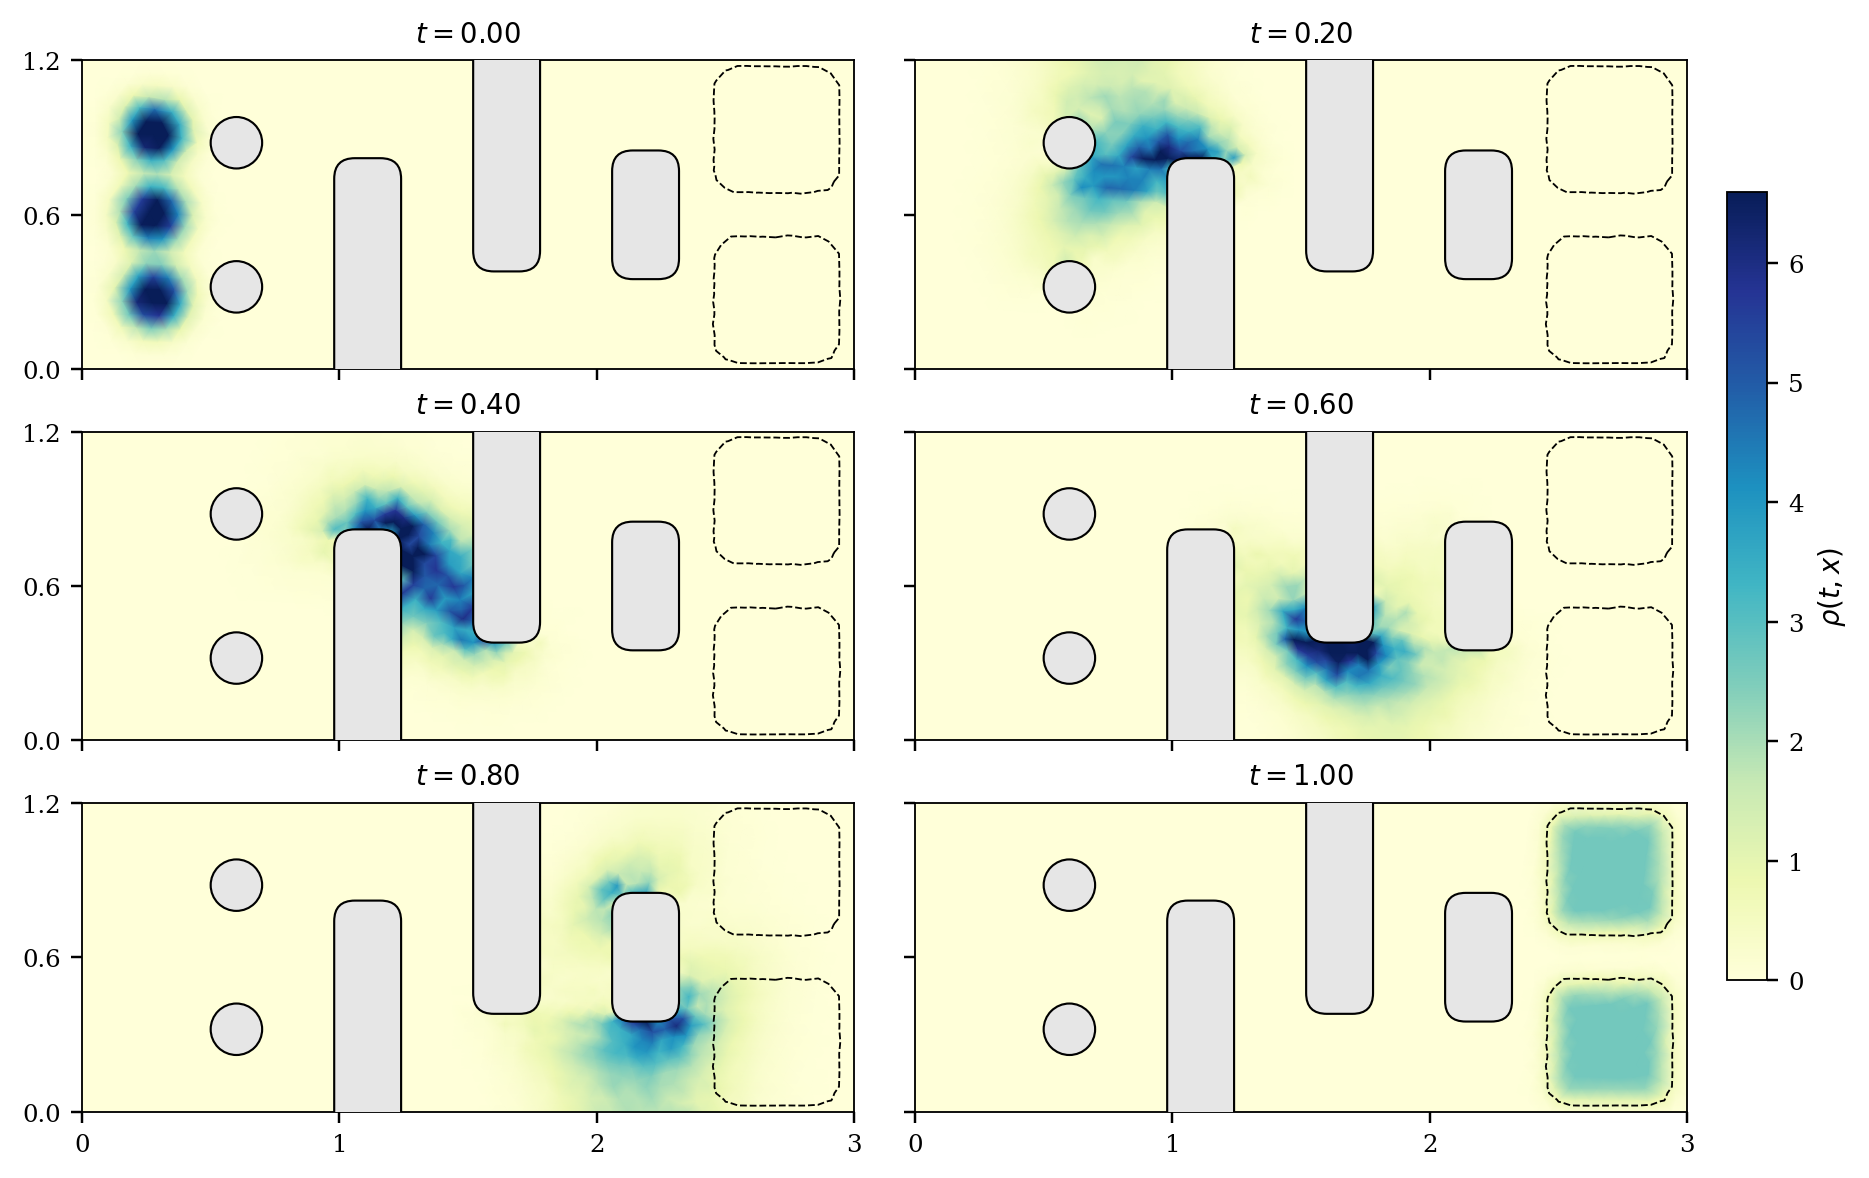
\includegraphics[width=\linewidth]{assets/fig1_density.png}
        \caption{finite-element nodal density $\rho (t,x)$}
        \label{subfig:a}
    \end{subfigure}
    \hfill
    \begin{subfigure}[b]{0.6\textwidth}
        \centering
        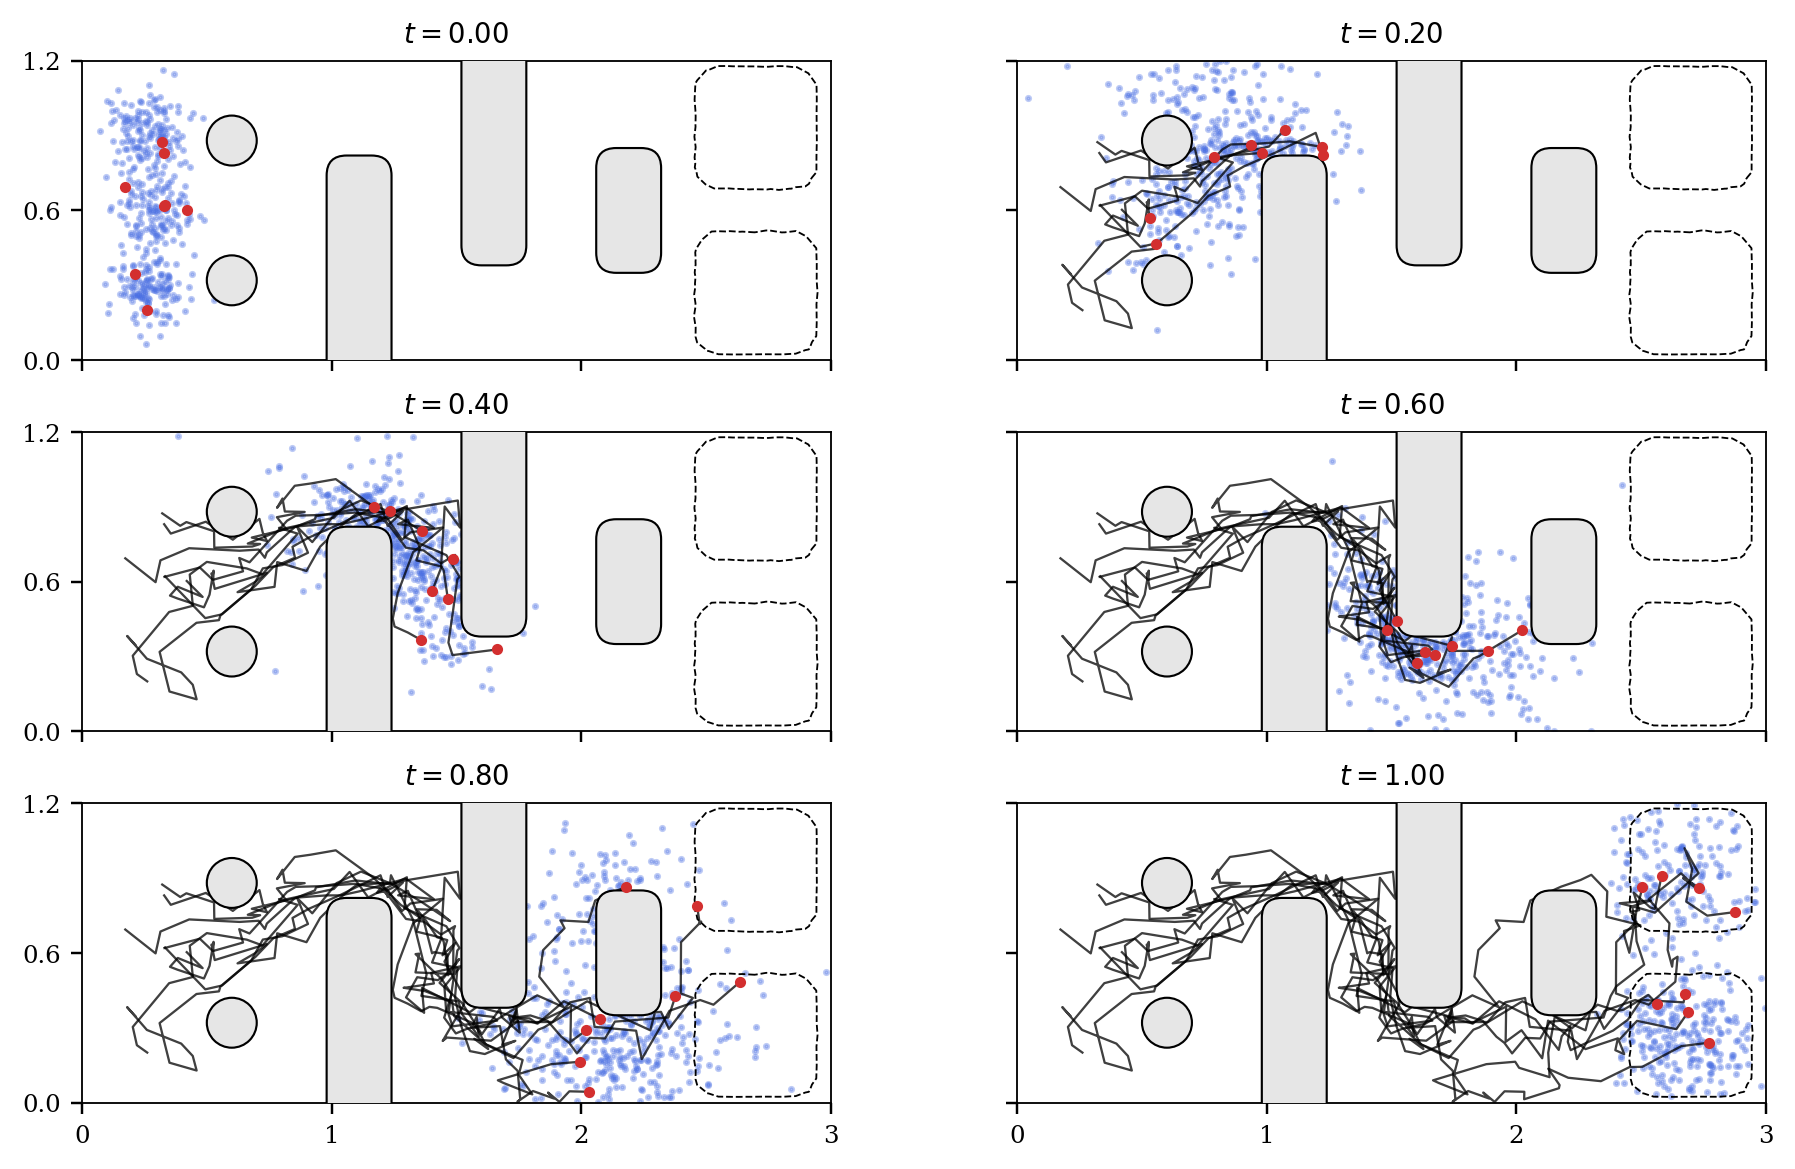
\includegraphics[width=\linewidth]{assets/fig1_particles.png}
        \caption{
            $N_{p} =1600$ independent Brownian particles with 8 highlighted sample paths.}
        \label{subfig:b}
    \end{subfigure}
    \caption{
        Illustrates the approximated density flow solution $\rho (t,x)$ alongside controlled 
        Euler--Maruyama particle trajectories for baseline parameters $\kappa =0.12$, 
        $N_{t} =50$, and $h_{\max} =0.06$ ($N=1388$ nodes). The outer iterate is with 
        damping factor $\theta =0.65$ converges in $n=22$ iterations and attained  
        $L^{1}$ density residual of $\| \Delta \rho ^{22} \| _{L^{1}} =1.156\times 
        10^{-8}$ ($\| \Delta \rho ^{22} \| _{L^{\infty }} =3.515\times 10^{-6}$), a terminal 
        Wasserstein-2 particle discrepancy of $W_{2} =5.365\times 10^{-2}$, and a total 
        wall-clock execution time $155.47\text{ s}$.
    }
    \label{fig:density_particle_2d_illustrate}
\end{figure}

\begin{table}[htbp]
    \centering
    \begin{tabular}{rcccccc}
    \toprule
    $n$ & $\|\delta \rho^n\|_{L^1}$ & $\frac{\|\delta \rho^n\|_{L^1}}{\|\delta \rho^{n-1}\|_{L^1}}$ & $\|\rho_0^n - \mu_{\text{init}}\|_{L^1}$ & $\|\rho_T^n - \mu_{\text{targ}}\|_{L^1}$ & $W_2(\rho_T^n, \mu_{\text{targ}})$ & $\max_k |\log Z_k|$ \\
    \midrule
    1  & $1.048 \times 10^{0\phantom{-}}$  & ---    & $6.047 \times 10^{-1}$ & $5.614 \times 10^{-1}$ & $5.285 \times 10^{-1}$ & $2.101 \times 10^{-3}$ \\
    3  & $4.160 \times 10^{-1}$ & 0.3500 & $7.408 \times 10^{-2}$ & $6.877 \times 10^{-2}$ & $1.698 \times 10^{-1}$ & $4.163 \times 10^{-2}$ \\
    5  & $5.312 \times 10^{-2}$ & 0.3656 & $9.075 \times 10^{-3}$ & $8.424 \times 10^{-3}$ & $5.704 \times 10^{-2}$ & $3.031 \times 10^{-2}$ \\
    10 & $2.227 \times 10^{-3}$ & 0.3496 & $4.766 \times 10^{-5}$ & $4.425 \times 10^{-5}$ & $3.885 \times 10^{-3}$ & $2.865 \times 10^{-2}$ \\
    15 & $1.169 \times 10^{-5}$ & 0.3500 & $2.503 \times 10^{-7}$ & $2.324 \times 10^{-7}$ & $2.693 \times 10^{-4}$ & $2.864 \times 10^{-2}$ \\
    16 & $4.093 \times 10^{-6}$ & 0.3500 & $8.762 \times 10^{-8}$ & $8.133 \times 10^{-8}$ & $1.574 \times 10^{-4}$ & $2.864 \times 10^{-2}$ \\
    \bottomrule

    \end{tabular}
    \small
    \caption{
        Fixed-point convergence for baseline 2D maze experiment. Boundary marginal 
        $L^{1}$ errors are evaluated on the damped iterate $\rho ^{n} =(1-\theta )\rho ^{n-1} +\theta 
        \rho _{\mathrm{half}}^{n}$.
        every step.
    }
    \label{tab:fixed_point}
    \vspace{0.5em}
\end{table}

Firstly, the nonlinear outer iteration is isolated (consider fixed density) and 
focus purely on linear forward-backward components. Here the artificial construction 
of frozen fields $b( t,x) ,r( t,x)$ along with terminal 
$\varphi ( T,x)$ where 
$x=( x_{0} ,x_{1}) \in \mathbb{R}^{2}$ are as follow, :
\begin{equation}
b( t,x) =(\cos x_{1} ,\sin x_{0}) ,\ r( t,x) =\sin x_{0}\cos x_{1} ,\ \text{and} 
\ \cos \varphi ( T,x) =1+\cos x_{1}\cos x_{0} .
\end{equation}
However, closed form expression exists and so the reference $
\varphi _{\text{ref}}$ is computed with finer time-space grid. Doupling termporal 
reference grid from $640$ to $1280$ steps (for fixed 
casrse mesh with $h_{\text{max}} =0.0787$) alters $L^{2}$ 
weight by $7.741\times 10^{-1}$ due to secular spatial interpolation 
residue. And for $h_{\text{max}} =0.035$ coupling $
N_{t} =320$ to $640$ changes the field by $1.182\times 10^{-3}$. 
And changes spatial reference from $0.045$ to $0.035$ 
changes the field by $1.502\times 10^{-2}$. Thus the reported smaller 
error to reference is due to artifact. Given two successive refinement levels 
$m-1$ and $m$ the empirical order of convergence (EOC) 
is measure using $\text{EOC} =\log\left(\text{err}^{m} /\text{err}^{m-1}
\right) /\log\left( h_{\text{max}}^{m} /h_{\max}^{m-1}\right)$ and mass-weighted nodal norm 
(computed over reference node $i\in I_{\Delta x}$ are
\begin{equation*}
{\textstyle \mathrm{err}_{p} (\varphi )=\left(\sum _{i} m_{i} |\varphi _{\mathrm{interp}} 
(0,x_{i} )-\varphi _{\mathrm{ref}} (0,x_{i} )|^{p}\right)^{1/p} ,\ \ \mathrm{err}_{\infty } (\varphi )=\max_{i} |\varphi _{\mathrm{interp}} (0,x_{i} )-\varphi _{\mathrm{ref}} (0,x_{i} )|.}
\end{equation*}
Additionally the the adjoint property, $L^{1}$ and Wasserstein-2 are mornitored for 
terminal distribution matching. 


\begin{figure}[htbp]
  \centering
  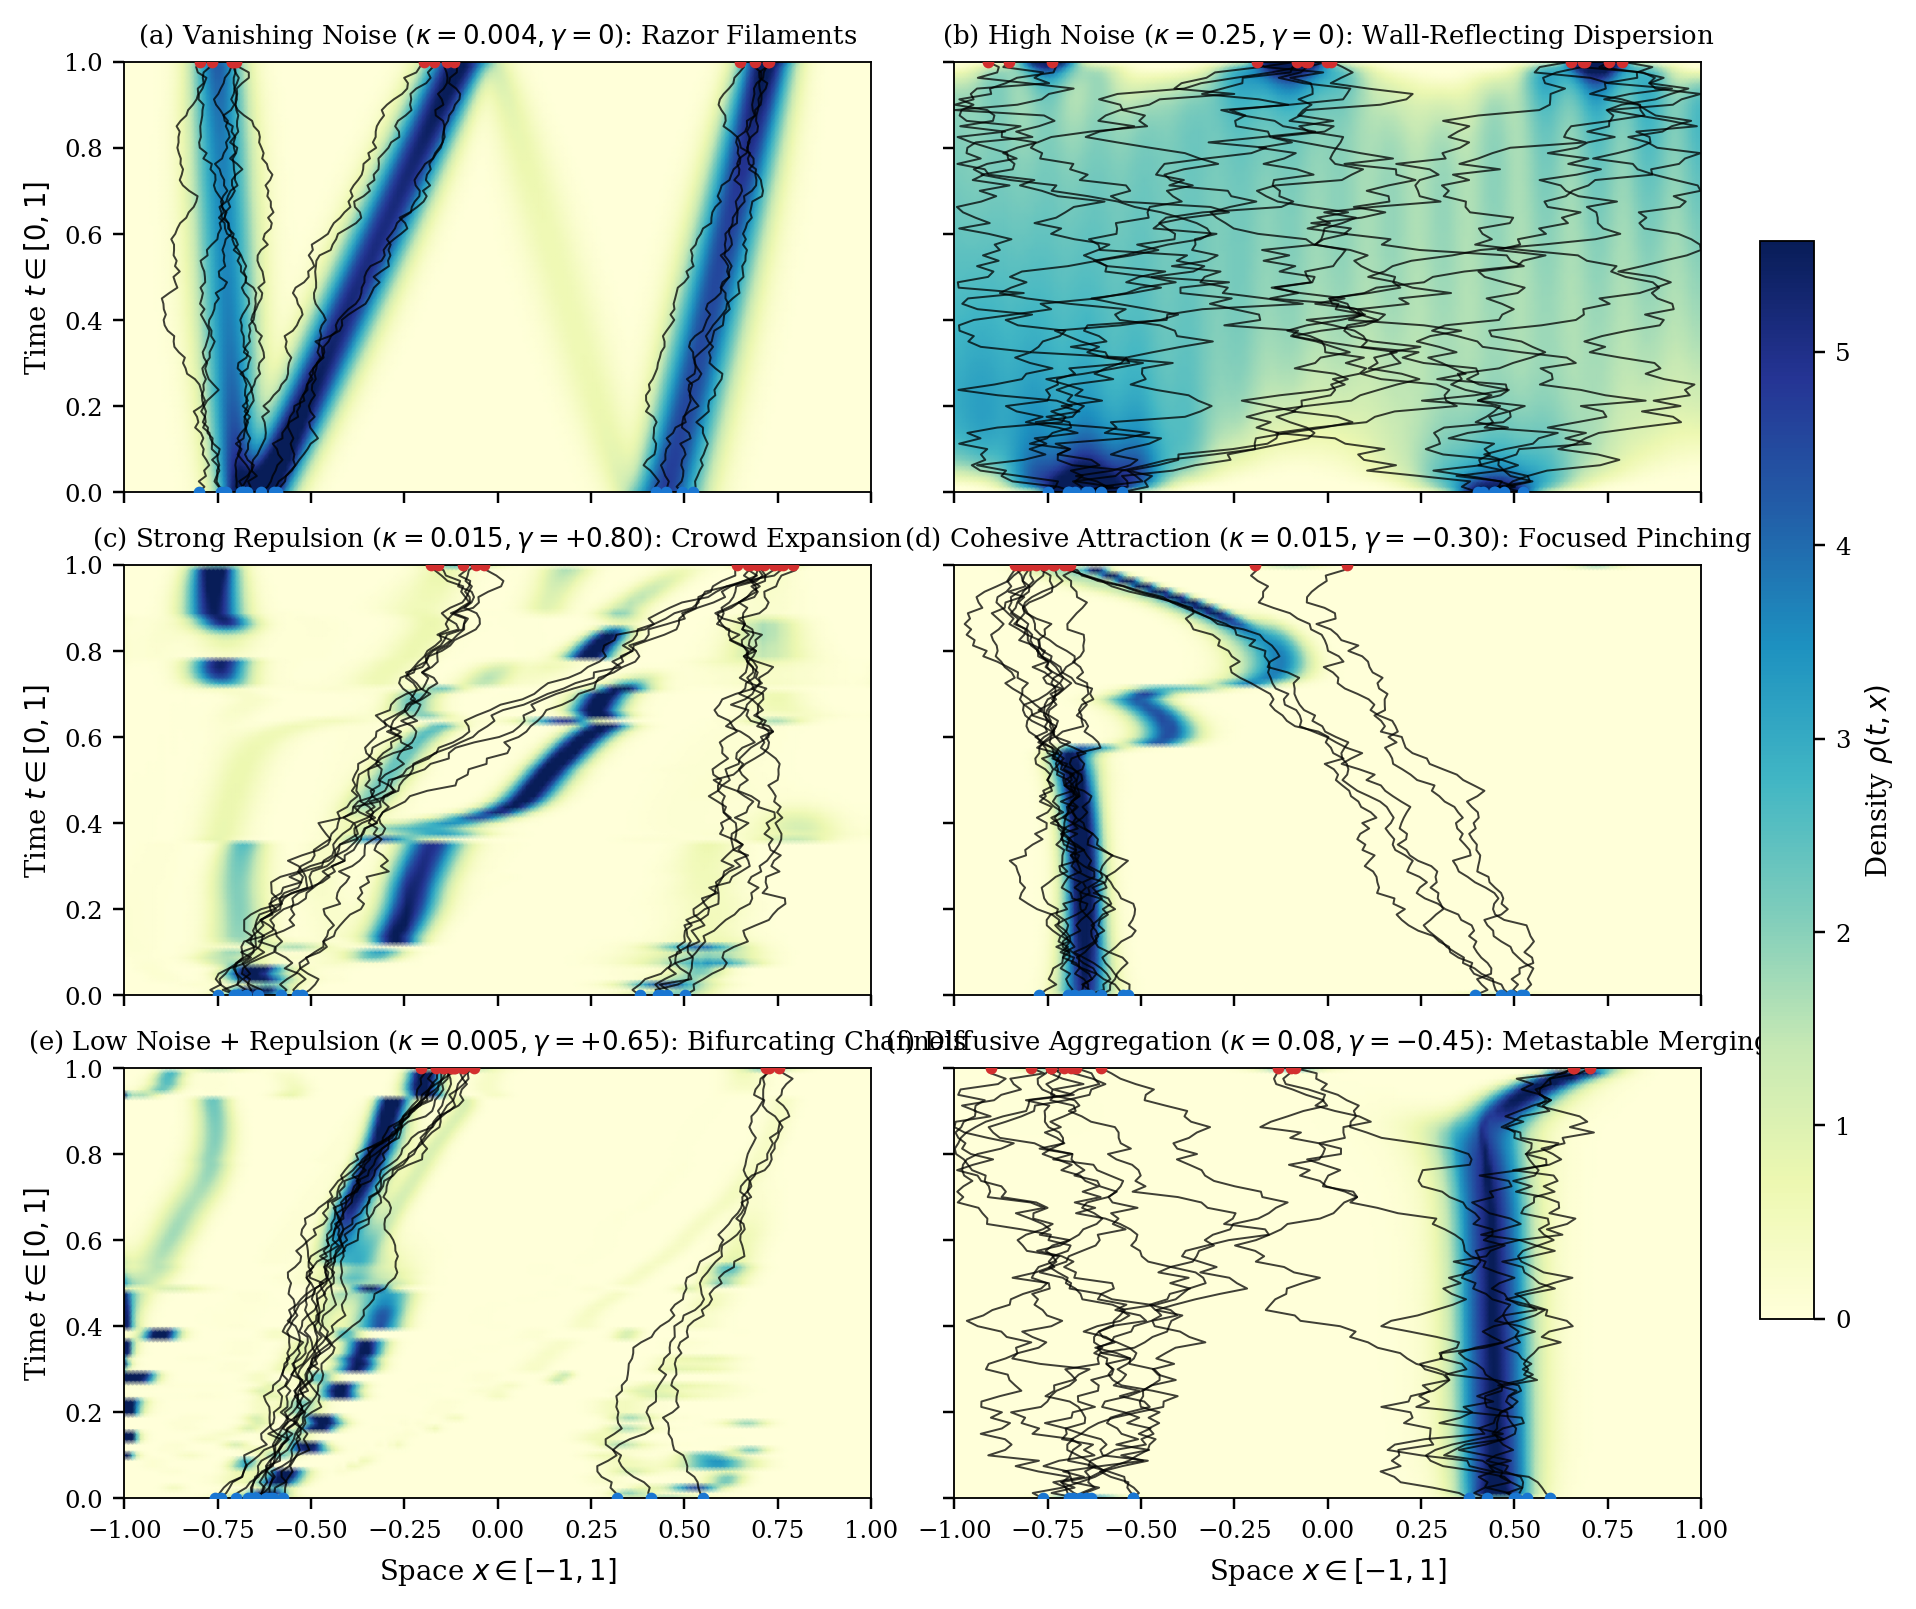
\includegraphics[width=0.92\linewidth]{assets/fig5_1d_extreme_transport} 
  \caption{One-dimensional space-time transport plans and particle
  trajectories under six extreme parameter regimes, illustrating
  deterministic filamentation ($\kappa = 0.004$), boundary-reflecting
  dispersion ($\kappa = 0.25$), repulsive crowd expansion ($\gamma = +0.80$),
  and attractive cohesive pinching ($\gamma = -0.30, -0.45$).}
  \label{fig:1d_extreme}
\end{figure}



\begin{figure}[htbp]
  \centering
  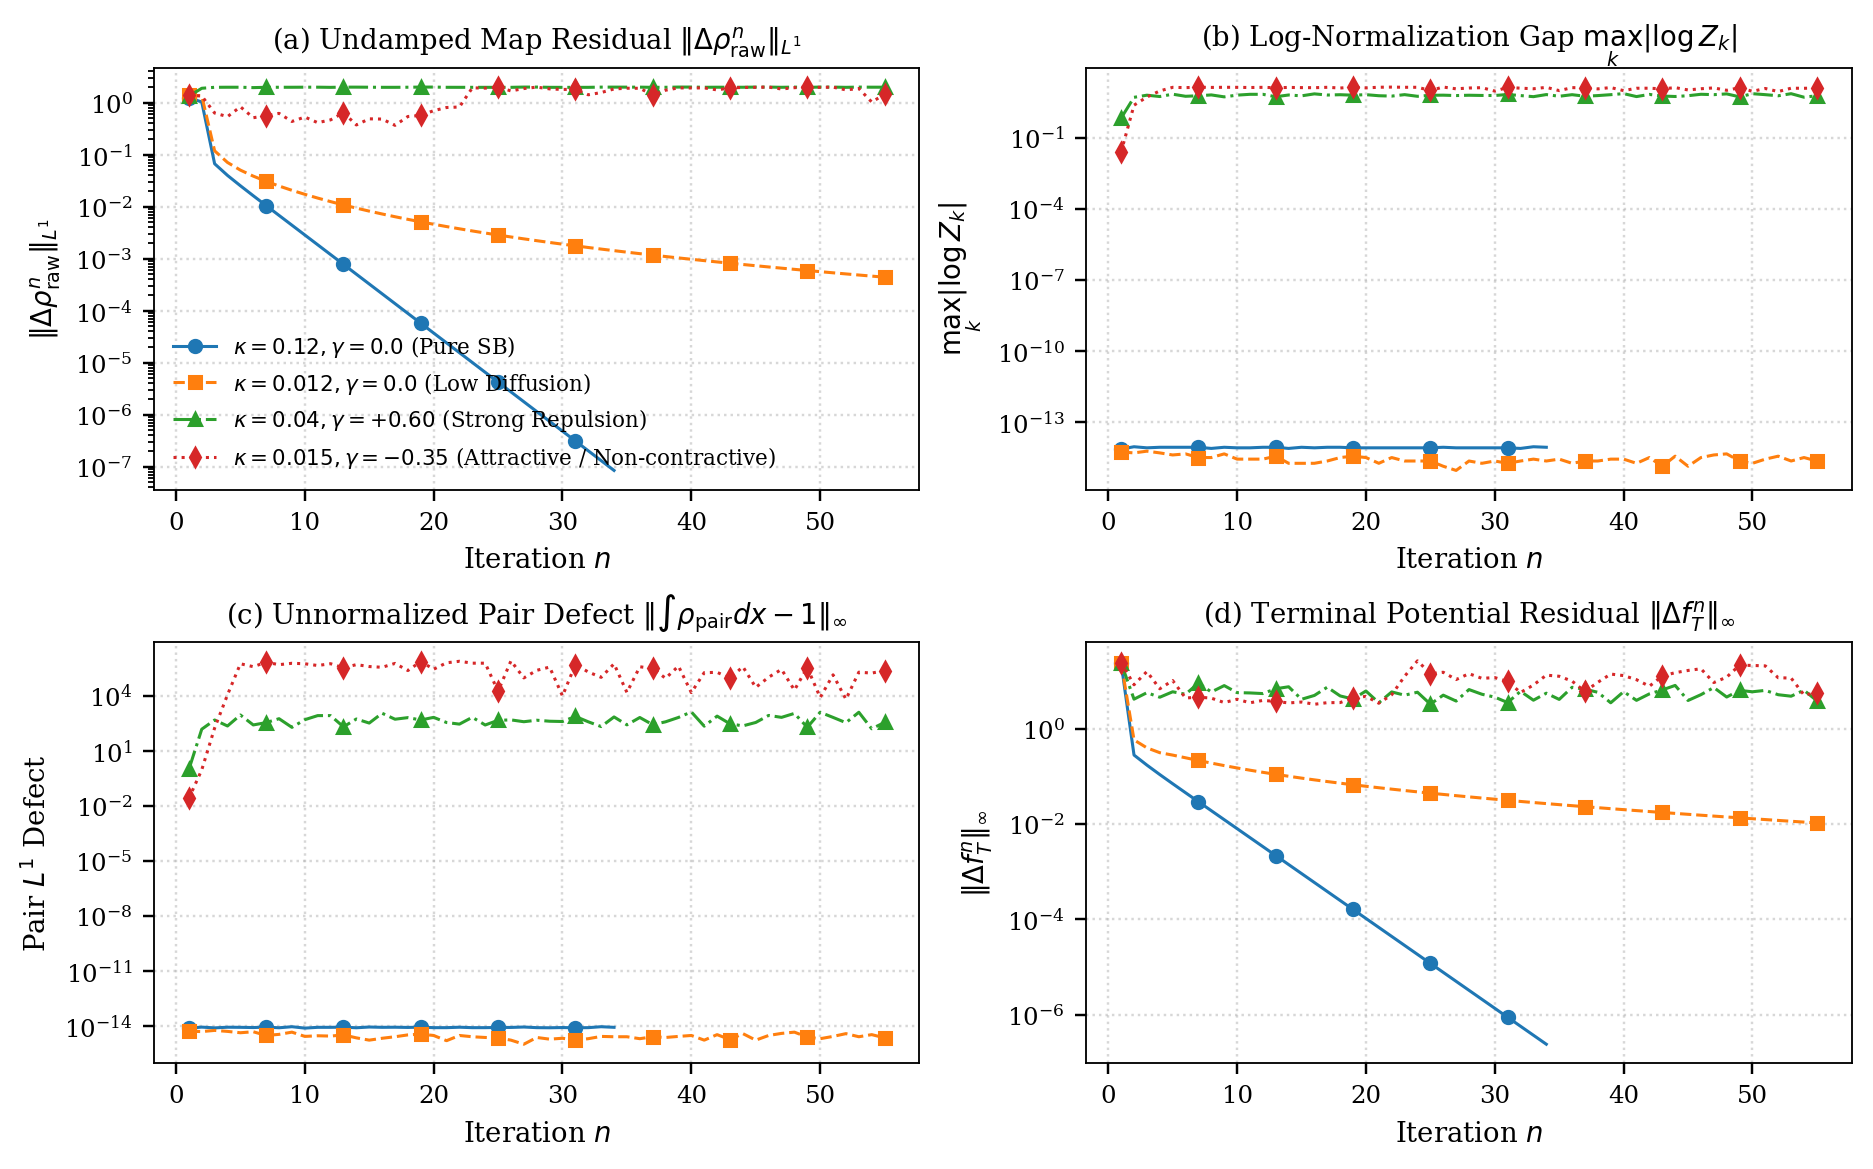
\includegraphics[width=0.92\linewidth]{assets/fig4_regime_diagnostics}
  \caption{Convergence diagnostics across $(\kappa, \gamma)$ regimes:
  (a)~undamped map residual $\|\Delta \rho_{\mathrm{raw}}^{n}\|_{L^{1}}$;
  (b)~log-partition gap $\max_{k} |\log Z_{k}|$; (c)~unnormalized pair-density
  $L^{1}$ defect; (d)~terminal potential residual $\|\Delta f_{T}^{n}\|_{\infty}$.}
  \label{fig:regime_diagnostics}
\end{figure}

Figure \ref{fig:regime_diagnostics} show 1-dim Mckean-Vlasov solution bridge under extreme diffusion from 
$\kappa =1$ to $\kappa =0.0004$ and repulsive interaction $\gamma _{0} =0$ to 
$\gamma _{0} =+0.8$ values. Under $\kappa \rightarrow 0$ the entropic interpolation 
reduce to narrow deterministic Monge-kantorivich optimal transport type that 
bifurcate sharply. The Péclet number $\text{Pe}_{h} =\Vert b\Vert _{\infty } 
y/( 2\kappa ) \gg 1$ is increased with slower contraction rate. For large 
$\gamma _{0}  >0$, high density is penalized since $\log W=-( E\star \rho ) /\kappa $ 
and forces mass to spread for unit of time rapidly toward every direction and 
approaching boundary $x=\pm 1$. This results in more frequent Skorokhod reflection, 
however constraction property still retained. This is possible when Skorkhod 
reflection is handled well, for instance that every escaping point is detected 
and correctly map back to feasible region $\mathcal{D}$ while retaining order of 
spatial accuracy. This this consideration, a substeping is employed. However for 
attractive force $\gamma _{0} < 0$ which makes particle tend toward dense 
concentrated area. When the ratio $| \gamma _{0}| /\kappa $ exceeds the critical 
bifurcation threshold (e.g. $\gamma _{0} =-0.35,\kappa =0.015$) the nonolocal 
feedback amplifies density perturbations and the normalized map enters a continually 
oscillatating cycle for all four metrics. 

\vspace{0.3cm}


The choice for $\displaystyle \Delta t$ in semi-lagrangian P1 scheme must takes into 
account (1) the local temporal splitting error and (2) the spatial interpolation error 
accumulated. Setting $\displaystyle \Delta t$ too small relative to 
$\displaystyle h_{\text{max}}$ in such a way that Courant number
 $\displaystyle C_{\text{CFL}} =\| b\| _{\infty } \Delta t/h_{\text{max}}\rightarrow 0$
  and diffusion characteristic jump size $\displaystyle \sqrt{6\kappa \Delta t} \ll h$, 
  the stochastic next point $\displaystyle x_{i} +b( x_{i}) \Delta t+\sqrt{2\kappa \Delta t} \xi _{q}$ 
  will be trapped inside their host element $\displaystyle K\in \mathrm{T}_{h}$. And 
  as $\displaystyle T/\Delta t\rightarrow \infty $ the repeated convex barycentratric 
  averaging (interpolation) within one same triangle acts as artificial numerical 
  viscosity of magnitude $\displaystyle h_{\text{max}}^{2} /\Delta t$. This is confirmed 
  in table \ref{tab:frozen_field} that under refining time grind on $\displaystyle h_{\text{max}} =0.0459$ the 
  EOC stagnates at 0.53 and 0.58 and turn negative EOC rates to -0.32 and -0.34. 


\begin{table}[htbp]
\centering
\small
\caption{Error convergence and computational runtime for the inner linear solve with frozen field.}
\label{tab:frozen_field}
\vspace{0.5em}
\begin{tabular}{cccccccc}
\toprule
$\Delta t$ & $h_{\max}$ & $|\mathcal{I}_{\Delta x}|$ & $e_\infty(\phi)$ & $e_2(\phi)$ & $e_2(\nabla \phi)$ & EOC & CPU (s) \\
\midrule
\multicolumn{8}{l}{\textit{Temporal Refinement (fixed $h_{\max} = 0.0459$)}} \\
0.2000 & 0.0459 & 3344 & $3.492 \times 10^{-1}$ & $1.288 \times 10^{-1}$ & $1.255 \times 10^{0\phantom{-}}$  & ---  & 0.37 \\
0.1000 & 0.0459 & 3344 & $2.073 \times 10^{-1}$ & $7.240 \times 10^{-2}$ & $6.747 \times 10^{-1}$ & 0.83 & 0.38 \\
0.0500 & 0.0459 & 3344 & $1.321 \times 10^{-1}$ & $4.125 \times 10^{-2}$ & $3.615 \times 10^{-1}$ & 0.81 & 0.25 \\
0.0250 & 0.0459 & 3344 & $7.355 \times 10^{-2}$ & $2.830 \times 10^{-2}$ & $2.054 \times 10^{-1}$ & 0.54 & 0.30 \\
0.0125 & 0.0459 & 3344 & $4.480 \times 10^{-2}$ & $1.966 \times 10^{-2}$ & $1.179 \times 10^{-1}$ & 0.53 & 0.44 \\
0.0083 & 0.0459 & 3344 & $3.468 \times 10^{-2}$ & $1.552 \times 10^{-2}$ & $7.961 \times 10^{-2}$ & 0.58 & 0.59 \\
0.0063 & 0.0459 & 3344 & $1.945 \times 10^{-2}$ & $1.228 \times 10^{-2}$ & $5.487 \times 10^{-2}$ & 0.81 & 0.74 \\
0.0042 & 0.0459 & 3344 & $1.385 \times 10^{-2}$ & $6.513 \times 10^{-3}$ & $2.527 \times 10^{-2}$ & 1.56 & 0.96 \\
0.0028 & 0.0459 & 3344 & $3.266 \times 10^{-3}$ & $2.512 \times 10^{-3}$ & $8.525 \times 10^{-3}$ & 2.35 & 1.25 \\
\midrule
\multicolumn{8}{l}{\textit{Spatial Refinement (fixed $\Delta t = 0.0063$)}} \\
0.0063 & 0.2019 & \phantom{0}324 & $1.829 \times 10^{-1}$ & $1.429 \times 10^{-1}$ & $4.237 \times 10^{-1}$ & ---  & 0.03 \\
0.0063 & 0.1576 & \phantom{0}455 & $1.084 \times 10^{-1}$ & $8.772 \times 10^{-2}$ & $3.019 \times 10^{-1}$ & 1.97 & 0.05 \\
0.0063 & 0.1067 & \phantom{0}678 & $7.907 \times 10^{-2}$ & $4.170 \times 10^{-2}$ & $1.900 \times 10^{-1}$ & 1.91 & 0.13 \\
0.0063 & 0.0787 & 1388           & $5.428 \times 10^{-2}$ & $1.258 \times 10^{-2}$ & $7.914 \times 10^{-2}$ & 3.93 & 0.24 \\
0.0063 & 0.0408 & 4567           & $2.794 \times 10^{-2}$ & $1.548 \times 10^{-2}$ & $6.703 \times 10^{-2}$ & -0.32 & 1.04 \\
0.0063 & 0.0068 & 142105         & $4.853 \times 10^{-2}$ & $2.818 \times 10^{-2}$ & $1.405 \times 10^{-1}$ & -0.34 & 37.61 \\
\midrule
\multicolumn{8}{l}{\textit{Spatiotemporal Refinement}} \\
0.0833 & 0.2019 & \phantom{0}324 & $2.405 \times 10^{-1}$ & $6.436 \times 10^{-2}$ & $2.932 \times 10^{-1}$ & ---  & 0.02 \\
0.0500 & 0.1576 & \phantom{0}455 & $1.856 \times 10^{-1}$ & $4.168 \times 10^{-2}$ & $2.423 \times 10^{-1}$ & 1.76 & 0.03 \\
0.0312 & 0.1067 & \phantom{0}678 & $1.413 \times 10^{-1}$ & $2.551 \times 10^{-2}$ & $1.715 \times 10^{-1}$ & 1.26 & 0.05 \\
0.0182 & 0.0787 & 1388           & $4.195 \times 10^{-2}$ & $1.450 \times 10^{-2}$ & $1.075 \times 10^{-1}$ & 1.85 & 0.14 \\
\bottomrule
\end{tabular}
\end{table}


\vspace{0.3cm}

Conversely, for too large $\displaystyle \Delta t$ relative to maze size can induce boundary 
penetration i.e. the characteristic displacement exceeds the "thickness" of boundary from 
which it penetrates. This also observed also as for non-convex and narrow interior holes, 
a single-step sign-distance projection (without taken into account the previous jump position) 
of $\displaystyle \hat{y} =y-2\chi ( y) \nabla \chi ( y)\mathbf{1}_{\left\{\chi ( y) < 0\right\}}$ 
fails to detect penetration if the half step lands entirely across the interior or project 
the foot onto the wrong face when crosses the medial axis. Fro instance suppose the wall 
of width $\displaystyle 0.26$ with $\displaystyle h_{\text{max}} =0.04$ and $\displaystyle 
C_{\text{CFL}} =10$, one stepproduces $\displaystyle \Delta x=C_{\text{CFL}} h_{\text{max}} 
=0.40 >0.26$ completely tunnelling trhough the hole without even triger subroutine check 
for $\displaystyle \chi < 0$. This phenomena is exacerbated as $\displaystyle t\rightarrow T$ 
by steep lagarithmic gradient $\displaystyle \nabla \log \varphi _{T}$ which, in this my setting 
for Gaussian-decayed distribution $\displaystyle \mu _{\text{targ}}$ for idstnace 
$\displaystyle d=0.5$ units from target, the terminal potential gradient pull strongly 
the particles with magnitude $\displaystyle \Vert \nabla \log \varphi _{T}\Vert $ approximately 
$\displaystyle d/\sigma _{T}^{2} =200$ times, where $\displaystyle \sigma _{T}^{2}$ is length 
strength parameter. This give exfective potential penalty of $\displaystyle 200\times 0.5$ and 
physical control drift $\displaystyle \alpha ^{*} =2\kappa \Vert \nabla \log \varphi _{T}\Vert =48$ 
unit per sec. However the domain must also be well-constructed and ensure there is path joining 
the target to initial distribution. 

The figure \ref{fig:disconnected_1d} illustrate this idea. For disconnected 
domain $\displaystyle [ -1,0] \cup [ 1,2]$ and large terminal 
gradient blow-up. Here $\displaystyle \mu _{\text{init}}$ concentrated around 
first half of the domain while $\displaystyle \mu _{\text{targ}}$ is on the otherside.
It is obvious that there is no solution such that $\displaystyle \rho _{T} =\mu _{\text{targ}}$ \ 
is any sense. Here the Skorokhond reflection at $\displaystyle \{-1,0\}$ and $\displaystyle \{1,2\}$ 
prevent characteristic path from crossing infeasible domain 
$\displaystyle \mathbb{R} -\mathcal{D} =( 0,1)$. And at the same time the terminal steep 
Gaussian tail distibution $\displaystyle \nabla \log \varphi _{T} \approx 
( x_{T} -x) /\sigma _{T}^{2} \in [ 355,591]$. For $\displaystyle t\ll T$ 
the (backward) heat semigroup $\displaystyle \varphi _{t} =\mathcal{U}_{t,T} \varphi _{T}$ 
exponentially damps non-constant mode on left half domain at the spectral-gap rate 
$\displaystyle e^{-\pi ^{2} \kappa ( T-t)}$ and maintain flat potential norm 
gradient $\displaystyle \Vert \nabla \log \varphi _{t}\Vert _{L^{\infty }\left(\text{left half of }
\mathcal{D}\right)} \ll 1$ over at the begining of $\displaystyle t$. As $\displaystyle t
\rightarrow T$ the control will try to match the terminal boundary condition and violently 
leat to frequent reflection. 

\vspace{0.3cm}

Note that the full nonlinear solver incured the discrete adjoint error for forward 
backward propagations almost to $\displaystyle 10^{-15}$ for all steps. Notably the 
damped outer density residual $\displaystyle \left\Vert \rho ^{n} -\rho ^{n-1}\right\Vert _{L^{1}}$ 
across different spatial operator splitting {\fontfamily{pcr}\selectfont Lie} vs 
{\fontfamily{pcr}\selectfont Strang} or choice of quadrature stecils including 
{\fontfamily{pcr}\selectfont axial4,axial5,gh9}, and monte-carlo {\fontfamily{pcr}\selectfont MC} 
give very identical convergence curve as illustrated in graph \ref{fig:fig2_splitting_stencils}.

\begin{figure}[htbp]
    \centering
    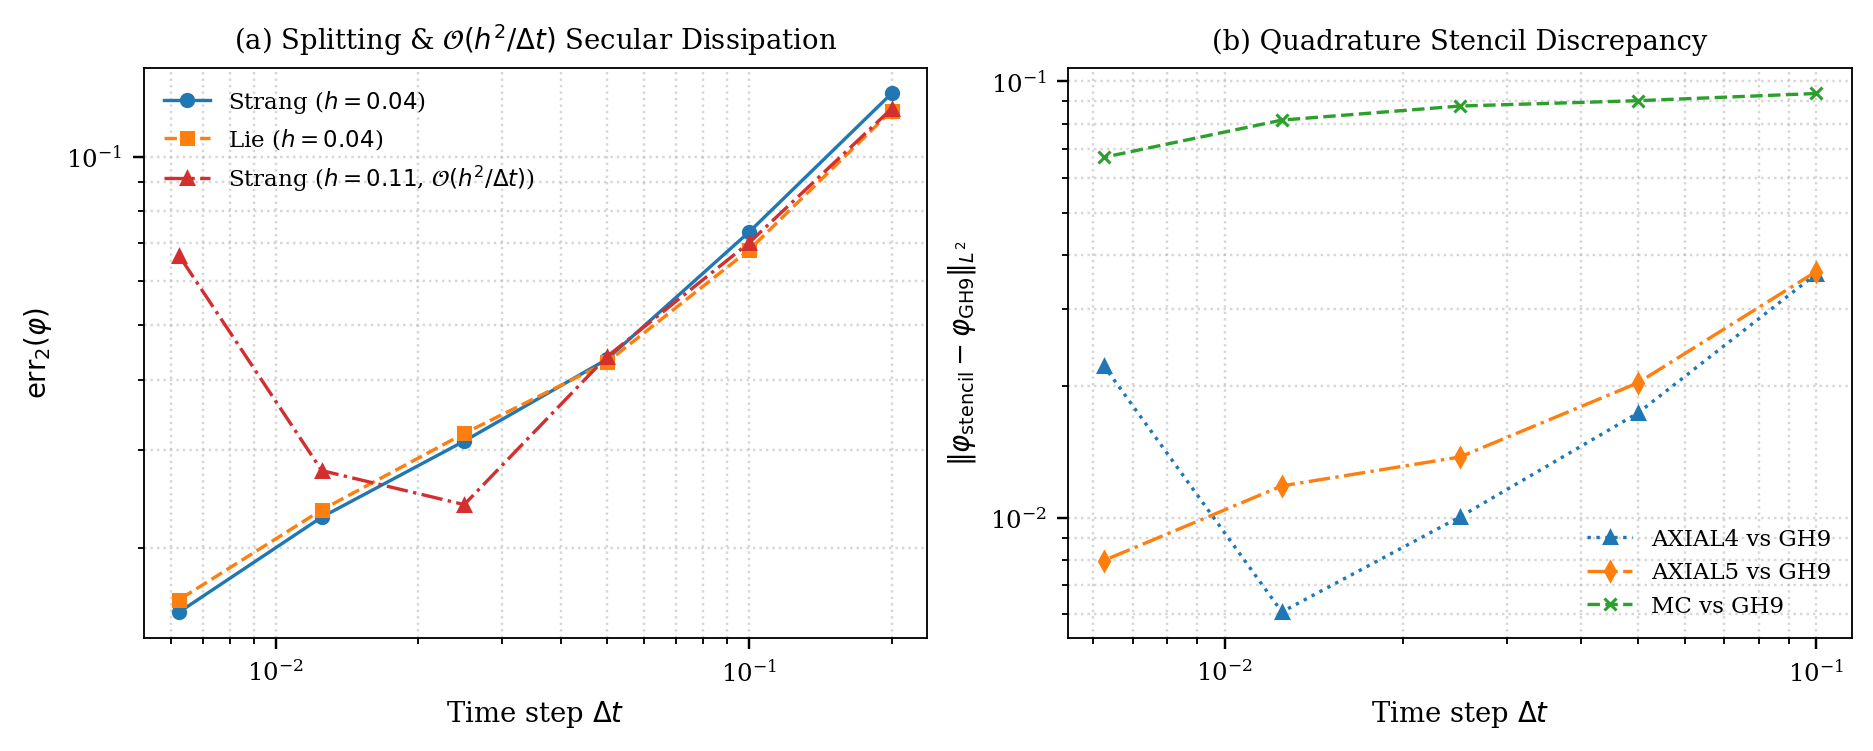
\includegraphics[width=0.92\linewidth]{assets/fig2_splitting_stencils}
    \caption{(a)~$\mathrm{err}_{2}(\varphi)$ versus $\Delta t$ illustrating
    second-order Strang versus first-order Lie scaling on a fine mesh
    ($h_{\max} = 0.04$) alongside the $\mathcal{O}(h^{2}/\Delta t)$ secular
    dissipation upturn on a coarse mesh ($h_{\max} = 0.11$);
    (b)~$L^{2}$ discrepancy of \texttt{axial4}, \texttt{axial5}, and
    $32$-sample antithetic Monte Carlo stencils relative to the tensor-product
    benchmark \texttt{GH9}.}
    \label{fig:fig2_splitting_stencils}
\end{figure}

Furthermore, adopting a log-domain implementation significantly eliminates floating-point 
overflow, i.e. setting $f=\log \varphi ,g=\log\hat{\varphi }$. This is particularly important 
for low diffusion level (e.g. $\kappa < 0.02$) which when evaluate raw density 
(which create order of $\exp\left( -\Vert x-y\Vert ^{2} /( 4\kappa \Delta t)\right) 
\sim e^{-100}$) \ causes underflow and division-by-zero in Sinkhorn scaling map. 
Using log-domain also helps with small negative oscillations near sharp boundary due 
to dispersion induced by P1 dispersion, which can cause Birkhoff-Bushell contraction 
to fail. In other word the normalize map $\displaystyle \rho =\exp (\log \rho -\log Z) >0$ 
is ensured by construction positive strictly.


\begin{figure}[htbp]
  \centering
  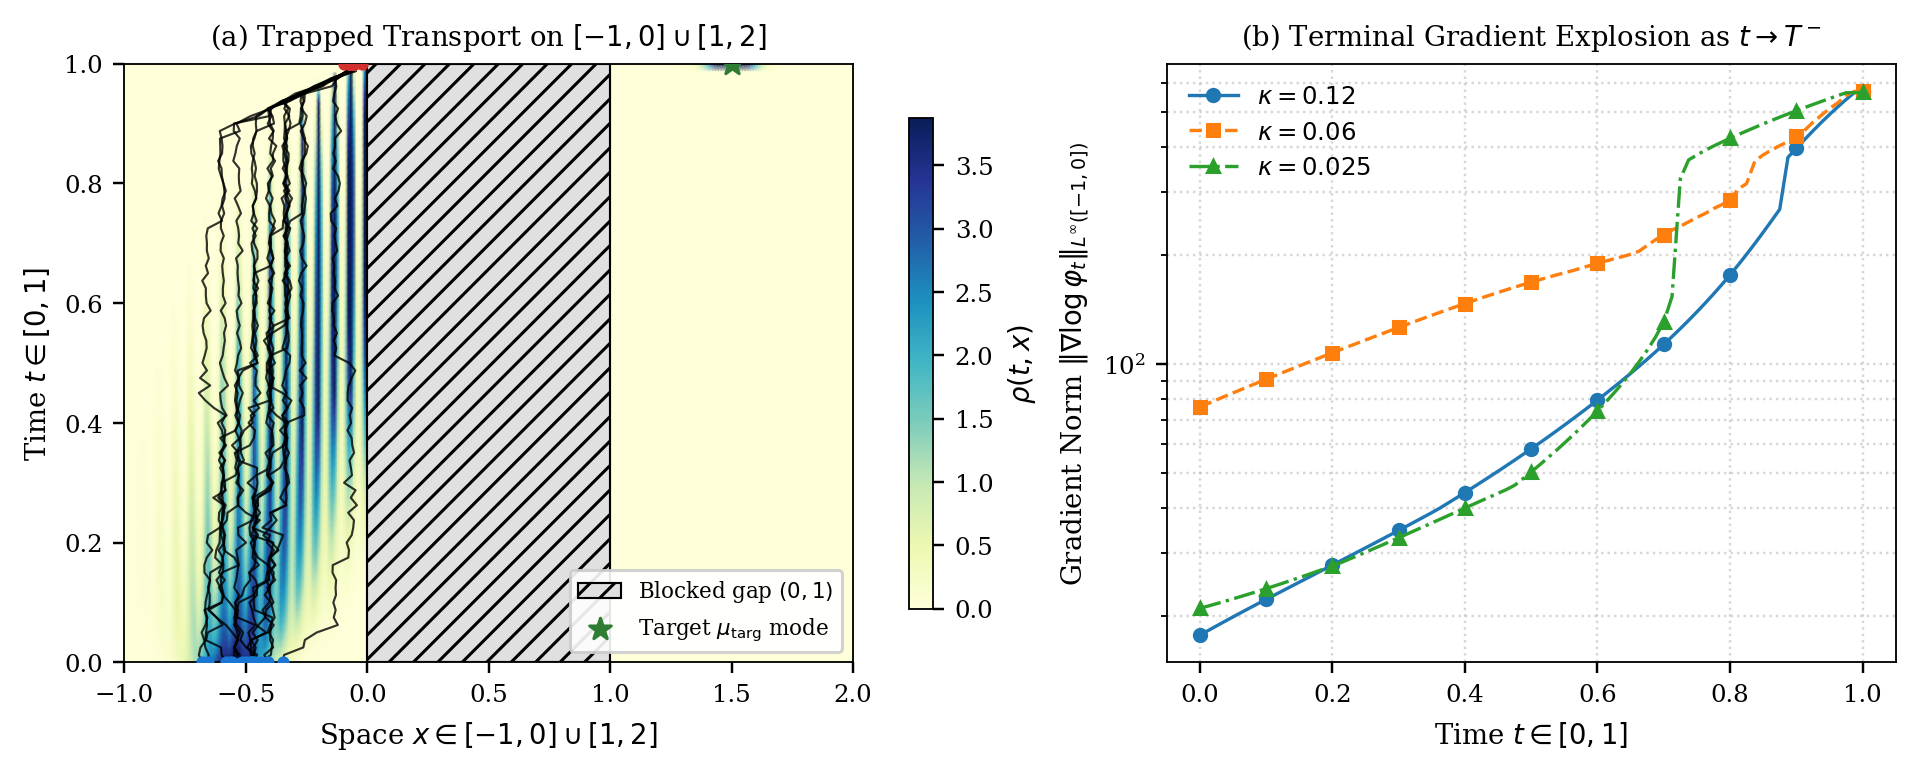
\includegraphics[width=0.92\linewidth]{assets/fig_disconnected_1d}
  \caption{Topological obstruction and terminal gradient blow-up on the
  disconnected domain $\Omega = [-1,0] \cup [1,2]$: (a)~particles initialized
  in $\mu_{\mathrm{init}}$ on $[-1,0]$ are blocked by the forbidden gap $(0,1)$
  and accumulate in a boundary layer at $x = 0^{-}$ near $t \to T^{-}$;
  (b)~temporal evolution of $\|\nabla \log \varphi_{t}\|_{L^{\infty}([-1,0])}$
  showing exponential blow-up as $t \to T^{-}$.}
  \label{fig:disconnected_1d}
\end{figure}


\section{Conclusion}



% \clearpage
% \bibliographystyle{plainnat}
% \bibliography{references}
\end{document}